\chapter{XÂY DỰNG GIAO DIỆN NGƯỜI DÙNG FRONTEND}

\section{Kiến trúc ứng dụng Single Page Application (SPA) với React và Vite}

Giao diện người dùng được xây dựng bằng React 18 với kiến trúc component hóa cao. Ứng dụng sử dụng React Router DOM để điều hướng trang không cần tải lại, kết hợp Axios Interceptor để tự động đính kèm mã JWT Bearer Token vào tiêu đề Authorization của mọi yêu cầu gửi đến Backend.

Hệ thống hỗ trợ cơ chế tự động chuyển hướng về trang Đăng nhập khi token hết hạn (HTTP 401), bảo đảm an toàn bảo mật cho phiên làm việc.

\section{Giao diện xác thực đăng nhập bảo mật}

Trang đăng nhập được thiết kế theo phong cách tối giản, hiện đại với tông màu xanh than chuyên nghiệp. Form đăng nhập có cơ chế kiểm tra tính hợp lệ dữ liệu trực tiếp trên máy khách (Client-side validation) và hiển thị thông báo lỗi rõ ràng khi thông tin đăng nhập không chính xác.

Giao diện đăng nhập thực tế của hệ thống được thể hiện tại Hình 10.1.

\begin{figure}[h!]
\centering
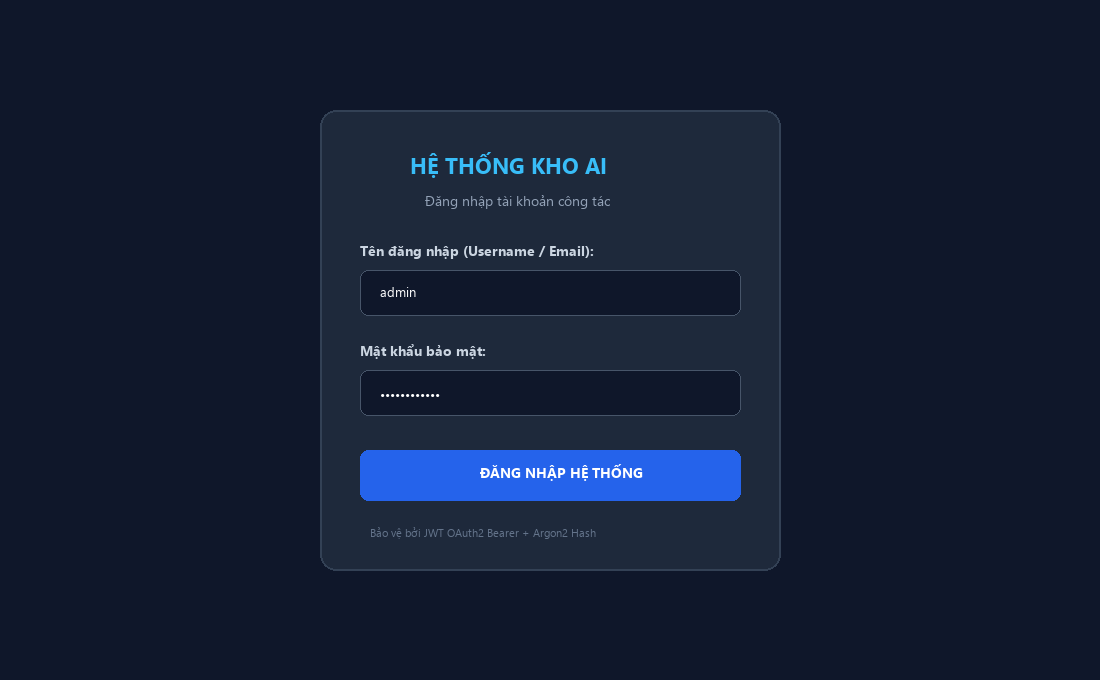
\includegraphics[width=0.92\textwidth]{figures/screenshot_login.png}
\caption{Giao diện Đăng nhập hệ thống bảo mật JWT OAuth2}
\end{figure}

\section{Giao diện Bảng điều khiển KPI Dashboard trực quan}

Bảng điều khiển KPI (Dashboard) là nơi cung cấp cái nhìn toàn cảnh về tình hình kho hàng cho các nhà quản lý trong thời gian thực. Màn hình bao gồm 6 thẻ chỉ số chủ chốt: Tổng số mặt hàng, Tổng tồn kho thực tế, Tổng định giá vốn tồn kho, Số mặt hàng sắp hết dưới ngưỡng an toàn, Lượng xuất 30 ngày và Lượng nhập 30 ngày, kết hợp biểu đồ cột thể hiện biến động xuất nhập.

Giao diện Bảng điều khiển KPI được trình bày tại Hình 10.2.

\begin{figure}[h!]
\centering
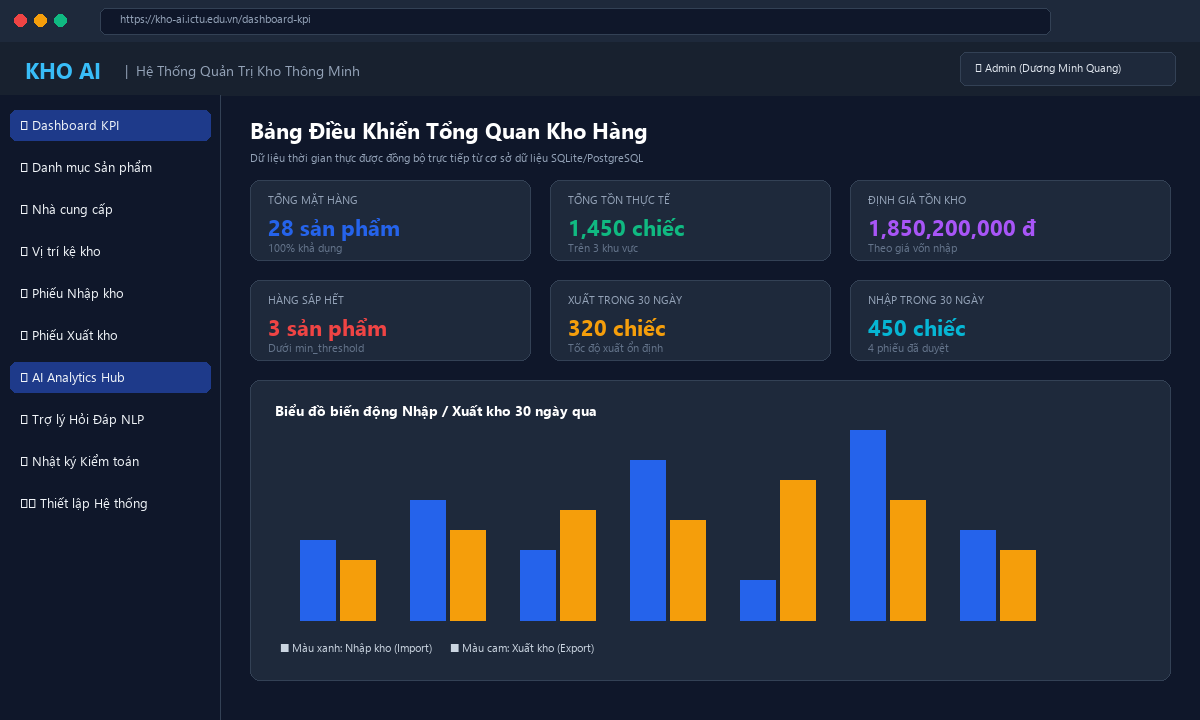
\includegraphics[width=0.92\textwidth]{figures/screenshot_dashboard.png}
\caption{Giao diện Bảng điều khiển KPI Dashboard kho hàng thời gian thực}
\end{figure}

\section{Giao diện Phân tích Trí tuệ Nhân tạo (AI Analytics Hub)}

Trung tâm phân tích AI (AI Analytics Hub) là tính năng vượt trội của hệ thống, cung cấp các tab chức năng: Báo cáo xuất nhập tồn, Gợi ý kế hoạch tái đặt hàng và Cảnh báo bất thường. Số liệu phân tích được trình bày dưới dạng bảng dữ liệu trực quan với các màu sắc cảnh báo rõ ràng (Đỏ: Hết hàng, Vàng: Dưới tồn, Xanh: Tồn an toàn).

Giao diện Trung tâm phân tích AI được thể hiện tại Hình 10.3.

\begin{figure}[h!]
\centering
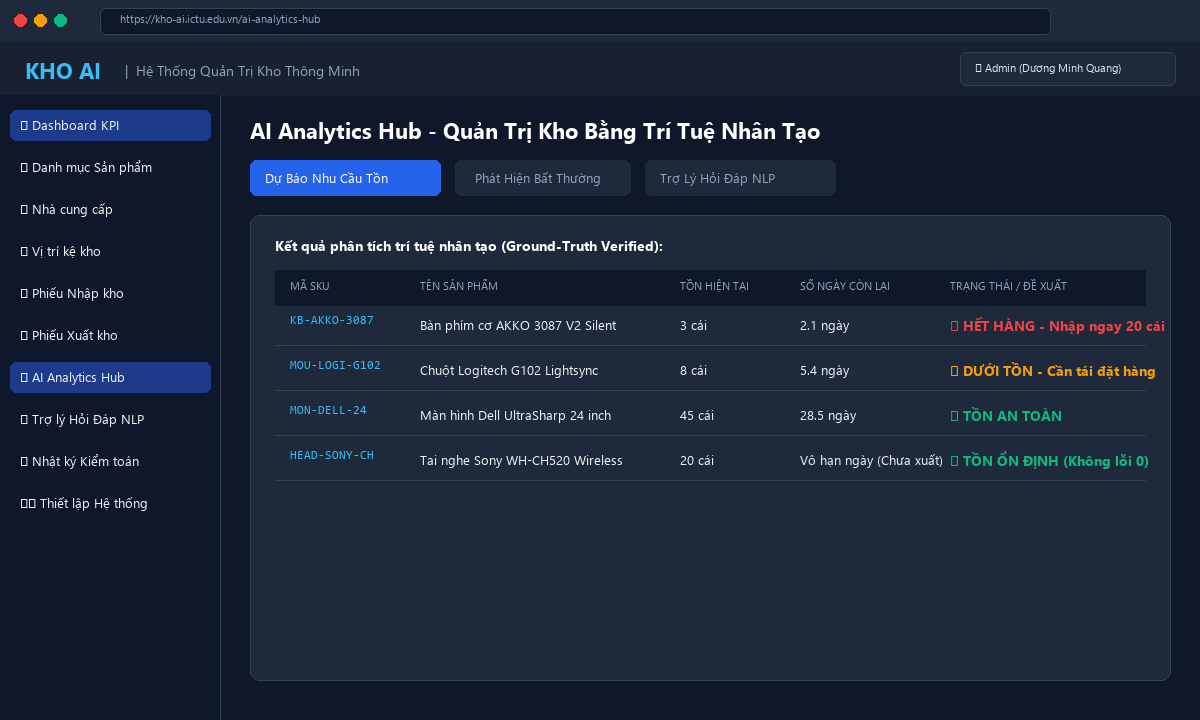
\includegraphics[width=0.92\textwidth]{figures/screenshot_ai_report.png}
\caption{Giao diện AI Analytics Hub hiển thị kết quả phân tích và dự báo tồn kho}
\end{figure}

\section{Giao diện Trợ lý thông minh hỏi đáp bằng tiếng Việt tự nhiên}

Giao diện trợ lý ảo được thiết kế tương tự các ứng dụng nhắn tin hiện đại. Người dùng có thể nhập câu hỏi nghiệp vụ vào khung chat và nhận về câu trả lời được định dạng Markdown chuẩn đẹp, kèm các bảng số liệu chi tiết và đề xuất hành động nghiệp vụ tiếp theo.

Giao diện Trợ lý hỏi đáp AI được minh họa tại Hình 10.4.

\begin{figure}[h!]
\centering
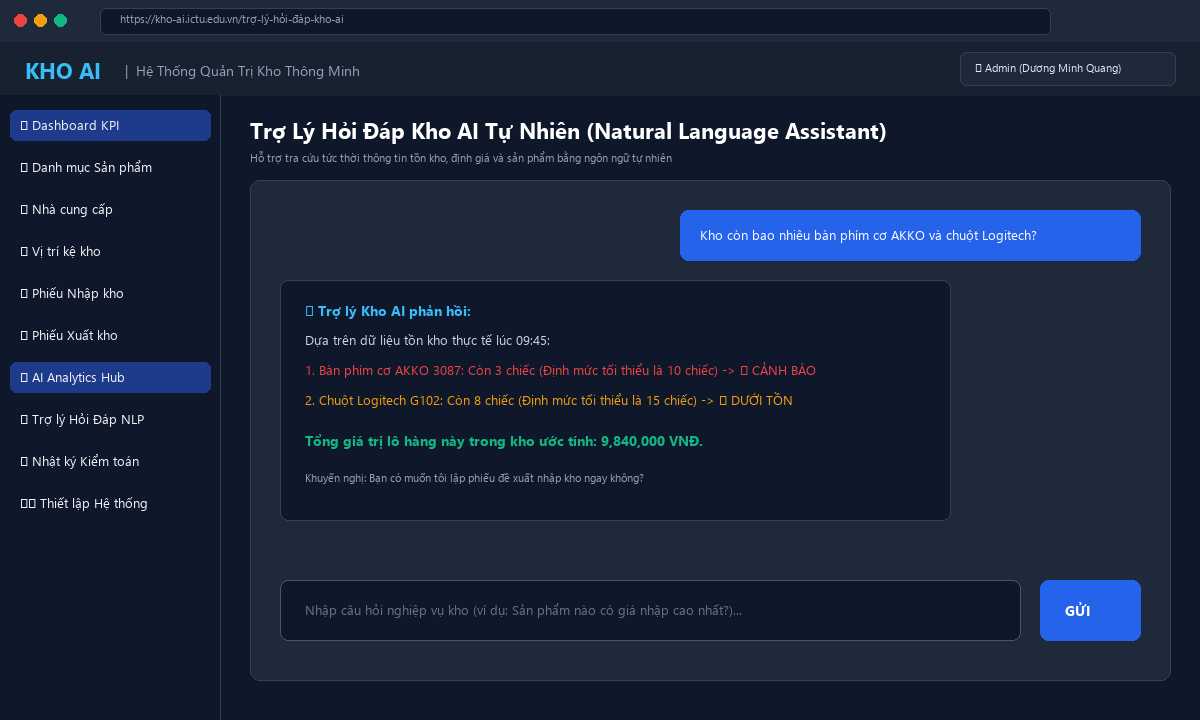
\includegraphics[width=0.92\textwidth]{figures/screenshot_ai_assistant.png}
\caption{Giao diện Trợ lý AI Hỏi Đáp ngôn ngữ tự nhiên về tình trạng kho}
\end{figure}

\section{Giao diện Quản lý danh mục Sản phẩm và dữ liệu Master}

Màn hình quản lý sản phẩm cho phép thủ kho tra cứu nhanh theo mã SKU hoặc tên sản phẩm, hiển thị đầy đủ thông tin đơn vị tính, giá vốn, giá bán niêm yết, định mức tồn an toàn và số lượng tồn hiện tại trong kho, hỗ trợ thêm mới và cập nhật sản phẩm nhanh chóng.

Giao diện Quản lý sản phẩm được thể hiện tại Hình 10.5.

\begin{figure}[h!]
\centering
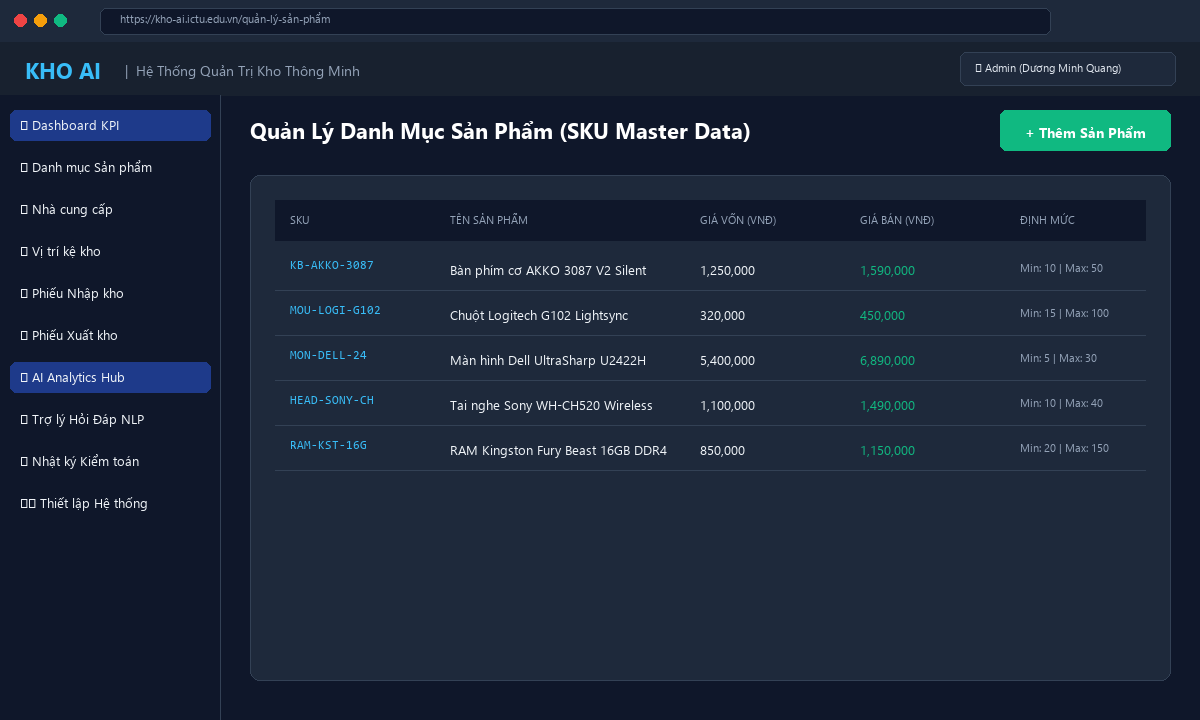
\includegraphics[width=0.92\textwidth]{figures/screenshot_products.png}
\caption{Giao diện Quản lý Danh mục Sản phẩm (SKU Master Data)}
\end{figure}

